%% LaTeX2e class for student theses
%% sections/content.tex
%% 
%% Karlsruhe Institute of Technology
%% Institute for Program Structures and Data Organization
%% Chair for Software Design and Quality (SDQ)
%%
%% Dr.-Ing. Erik Burger
%% burger@kit.edu
%%
%% Version 1.3, 2016-12-29

\chapter{PCM Extension}
\label{ch:pcmExtension}

\section{General}
\label{sec:pcmExtension:general}

As mentioned in Foundational Work the Palladio Component Model (\autoref{sec:Foundations:pcm}) was designed for early architectural performance analysis. On this basis, the PCM was modified many times to fulfil many adjacent tasks. Contrary to a modification, we decided to extend the existing PCM meta-model. This enables us to keep compatible with the existing Palladio Models and other Palladio applications.

The standard Palladio meta-model is insufficient for privacy compliance analysis. To save the required information, an extension is the best practice approach. The extension was designed be as minimal invasive as possible, to keep the adoption effort for existing Palladio models to a minimum.

The concept was described in \autoref{sec:PrivacyConcept:pcm}.

\begin{figure}[h]
	\centering
	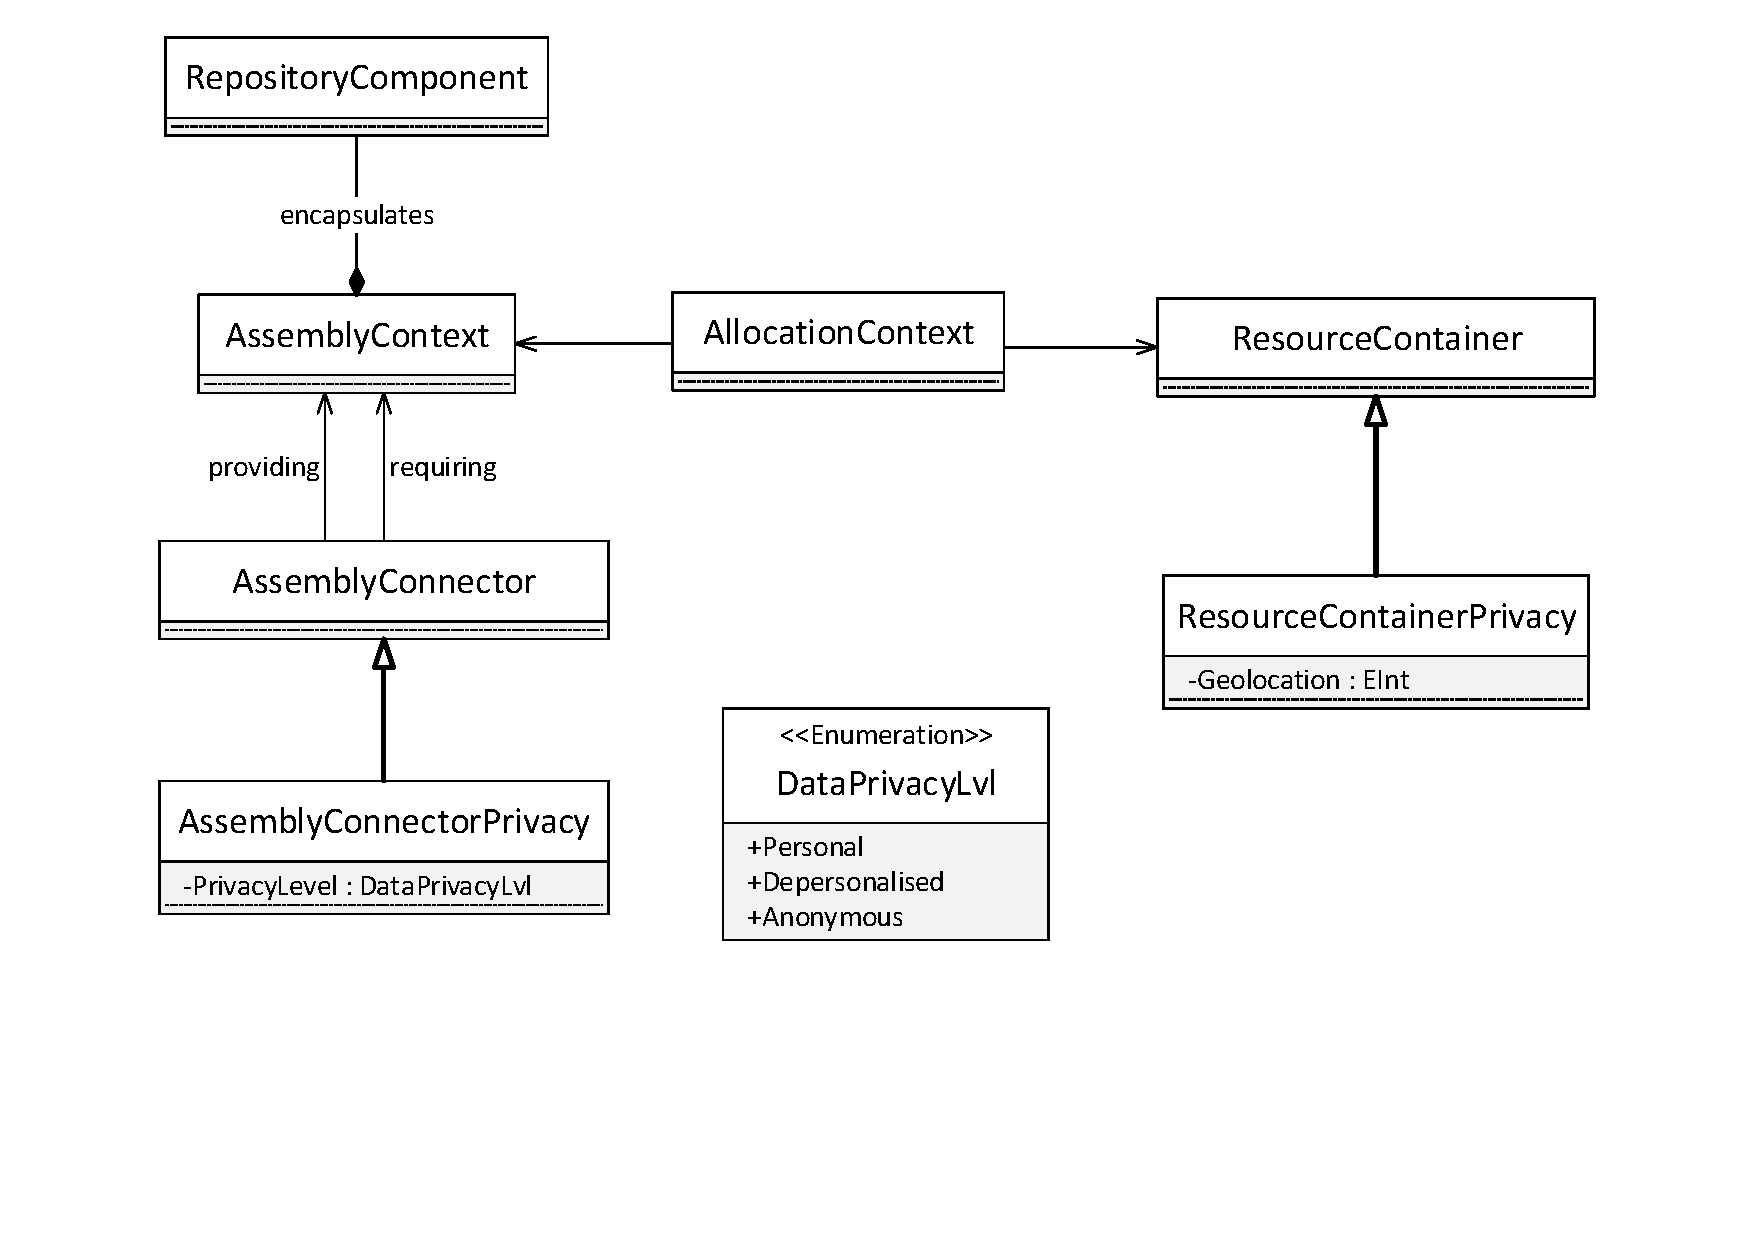
\includegraphics[trim = 20mm 50mm 20mm 05mm, clip, width=0.85\textwidth]{graphs/pcm_privacy_meta}
	\caption{Deployment analysis result}
	\label{fig:pcmExtension:meta}
\end{figure}


\section{Implementation}
\label{sec:pcmExtension:impl}

The Palladio meta-model was modelled with the Eclipse Modeling Framework [EMF]. So, our extension, namely \textit{PCM Privacy}, is also modelled with EMF and references the original Palladio meta-model. The required classes were extended in corresponding sub-packages.

As described in \autoref{sec:PrivacyConcept:pcm}, we need to save a servers geo-location. The Resource Container was extended and the attribute \textit{Geolocation} added. The extended element is named \textit{Resource Container Privacy}. The geo-location itself is saved as an EInt Ecore type, a standard integer, encoded in the ISO country code (ISO 3166-1 \cite{Wikipedia.ISO_3166}).

The \textit{Assembly Connector Privacy} is the extension of the Assembly Connector and saves the data privacy categorization. The attribute is designed as an EEnum Ecore type, with the values Personal, Depersonalized, Anonymized. The value Personal is set as default. \autoref{fig:pcmExtension:meta} shows a simplified PCM meta-model with the three added privacy elements.


%To ensure privacy compliance, the geo-location of a component is required. In Palladio a system component is deployed onto Resource Containers. So, the Resource Container is the model equivalent of a physical/virtual server. This makes it the conceptual storage unit for the geo-location. Thus, a components geo-location can be determined via the Resource Container it is deployed on, namely the deployment model. The geo-location itself is saved as an EInt Ecore type, a standard integer, encoded in the ISO country code.

%A PCM is designed in multiple steps. Initially, interfaces for the components must be designed, followed by components and composite components. These are saved in the PCM repository model. The actual PCM system model, representing the software system, references components from the repository model. These are then connected via Assembly Connectors. While components and composed components in the repository must be deployed as a whole onto one Resource Container, components which are connected via Assembly Connectors in the system model, can be deployed on different Resource Containers. This makes the Assembly Connector the optimal model entity for categorizing the exchanged data regarding the privacy level. 

